\begin{figure}
    \centering
    \begin{minipage}{\linewidth}
            {
                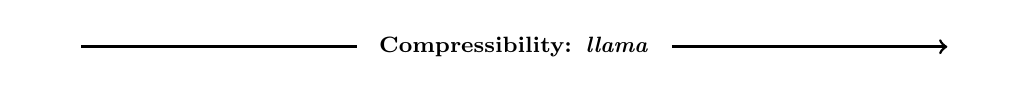
\begin{tikzpicture}
                    \draw[-, line width=1pt] (-5.5,0) -- (-2.0,0);
                    \node[text width=\linewidth, align=center] at (0,0) {
                        \footnotesize
                        \text{\textbf{Compressibility: \emph{llama}}}
                    };
                    \draw[->, line width=1pt] (2.0,0) -- (5.5,0);
                \end{tikzpicture} \\
            }
        \lfbox[
            border-width=2pt,
            padding-top=0pt,
            padding-bottom=0pt,
            padding-left=-2.6pt,
            padding-right=-2.5pt,
        ]{
            \includegraphics*[width=0.1684\linewidth]{teaser/jpeg-ppo-llama/0.jpg}
            \hspace{-0.7em}
            \includegraphics*[width=0.1684\linewidth]{teaser/jpeg-ppo-llama/9.jpg}
            \hspace{-0.7em}
            \includegraphics*[width=0.1684\linewidth]{teaser/jpeg-ppo-llama/39.jpg}
            \hspace{-0.7em}
            \includegraphics*[width=0.1684\linewidth]{teaser/jpeg-ppo-llama/59.jpg}
            \hspace{-0.7em}
            \includegraphics*[width=0.1684\linewidth]{teaser/jpeg-ppo-llama/79.jpg}
            \hspace{-0.7em}
            \includegraphics*[width=0.1684\linewidth]{teaser/jpeg-ppo-llama/99.jpg}
        }
    \end{minipage}
    \vspace{0.1em} \\
    \begin{minipage}{\linewidth}
        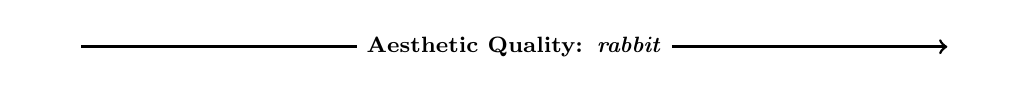
\begin{tikzpicture}
            \draw[-, line width=1pt] (-5.5,0) -- (-2,0);
            \node[text width=\linewidth, align=center] at (0,0) {
                \footnotesize
                \text{\textbf{Aesthetic Quality: \emph{rabbit}}}
            };
            \draw[->, line width=1pt] (2,0) -- (5.5,0);
        \end{tikzpicture} \\
        \lfbox[
            border-width=2pt,
            padding-top=0pt,
            padding-bottom=0pt,
            padding-left=-2.6pt,
            padding-right=-2.5pt,
        ]{
            \includegraphics*[width=0.1684\linewidth]{teaser/rabbit-aesthetic/0.jpg}
            \hspace{-0.7em}
            \includegraphics*[width=0.1684\linewidth]{teaser/rabbit-aesthetic/1.jpg}
            \hspace{-0.7em}
            \includegraphics*[width=0.1684\linewidth]{teaser/rabbit-aesthetic/2.jpg}
            \hspace{-0.7em}
            \includegraphics*[width=0.1684\linewidth]{teaser/rabbit-aesthetic/3.jpg}
            \hspace{-0.7em}
            \includegraphics*[width=0.1684\linewidth]{teaser/rabbit-aesthetic/4.jpg}
            \hspace{-0.7em}
            \includegraphics*[width=0.1684\linewidth]{teaser/rabbit-aesthetic/5.jpg}
        }
    \end{minipage}
    \vspace{0.1em} \\
    \begin{minipage}{\linewidth}
        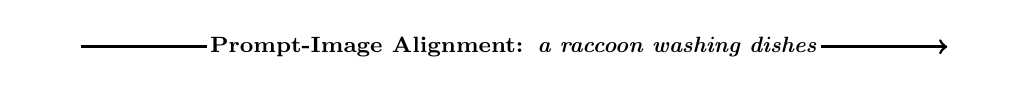
\begin{tikzpicture}
            \draw[-, line width=1pt] (-5.5,0) -- (-3.9,0);
            \node[text width=\linewidth, align=center] at (0,0) {
                \footnotesize
                \text{\textbf{Prompt-Image Alignment: \emph{a raccoon washing dishes}}}
            };
            \draw[->, line width=1pt] (3.9,0) -- (5.5,0);
        \end{tikzpicture} \\
        \lfbox[
            border-width=2pt,
            padding-top=0pt,
            padding-bottom=0pt,
            padding-left=-2.6pt,
            padding-right=-2.5pt,
        ]{
            \includegraphics*[width=0.1684\linewidth]{teaser/raccoon_dishes/0.jpg}
            \hspace{-0.7em}
            
\includegraphics[width=0.1684\linewidth]{teaser/raccoon_dishes/1.jpg}
            \hspace{-0.7em}
            \includegraphics*[width=0.1684\linewidth]{teaser/raccoon_dishes/2.jpg}
            \hspace{-0.7em}
            \includegraphics*[width=0.1684\linewidth]{teaser/raccoon_dishes/3.jpg}
            \hspace{-0.7em}
            \includegraphics*[width=0.1684\linewidth]{teaser/raccoon_dishes/4.jpg}
            \hspace{-0.7em}
            \includegraphics*[width=0.1684\linewidth]{teaser/raccoon_dishes/5.jpg}
        }
    \end{minipage}
    \caption{
        \textbf{(Reinforcement learning for diffusion models)}
            We propose a reinforcement learning algorithm, \methodours{}, for optimizing diffusion models on downstream objectives such as compressibility, aesthetic quality, and prompt-image alignment as determined by vision-language models. Each row shows a progression of samples for the same prompt and random seed over the course of training.
        }
    \vspace{-10pt}
\end{figure}